\documentclass[aspectratio=169,11pt]{beamer}

\usetheme{Madrid}
\usecolortheme{default}
\usefonttheme{professionalfonts}
\setbeamertemplate{navigation symbols}{}
\setbeamertemplate{footline}[frame number]

\usepackage{amsmath, amssymb, booktabs, graphicx}
\graphicspath{{../../assets/figures/}{assets/figures/}}

\title{Job Amenities and Compensating Differentials}
\subtitle{Labor I --- Week 7}
\author{Teaching deck draft}
\date{}

\begin{document}

\begin{frame}
  \titlepage
\end{frame}

\begin{frame}{Central question and motivation}
\begin{itemize}
    \item Week 7 asks how workers trade wages against nonwage job attributes.
    \item Jobs differ in safety, flexibility, predictability, commute burden, autonomy, and remote-work options.
    \item Wage data alone can therefore mismeasure welfare, sorting, and inequality.
\end{itemize}
\end{frame}

\begin{frame}{Week 6 to Week 7 bridge}
\begin{itemize}
    \item Week 6 showed that family structure changes the value of time and flexibility.
    \item Week 7 moves from household allocation to market equilibrium over wage-plus-amenity bundles.
    \item The same amenity can be worth more to workers facing care constraints, long commutes, or mobility frictions.
\end{itemize}
\end{frame}

\begin{frame}{Jobs as wage-plus-amenity bundles}
\[
V_i(w, a) = v_i(w) + \psi_i(a)
\]

\begin{itemize}
    \item Workers choose jobs, not wages in isolation.
    \item If \(a\) is a good, like schedule control or safety, workers may accept lower wages to get more of it.
    \item If \(a\) is a bad, like injury risk or unpredictability, wages must compensate at the margin.
\end{itemize}
\end{frame}

\begin{frame}{Rosen hedonic equilibrium}
\[
\frac{dw(a)}{da} = - \frac{V_a(w, a)}{V_w(w, a)}
\]

\begin{itemize}
    \item The slope of the wage schedule equals the worker's marginal willingness to trade wages for amenities.
    \item Better amenities can come with lower wages in equilibrium because workers value them directly.
    \item Observed slopes already reflect sorting across workers with different tastes and outside options.
\end{itemize}
\end{frame}

\begin{frame}{Hedonic wage-amenity equilibrium}
\begin{center}
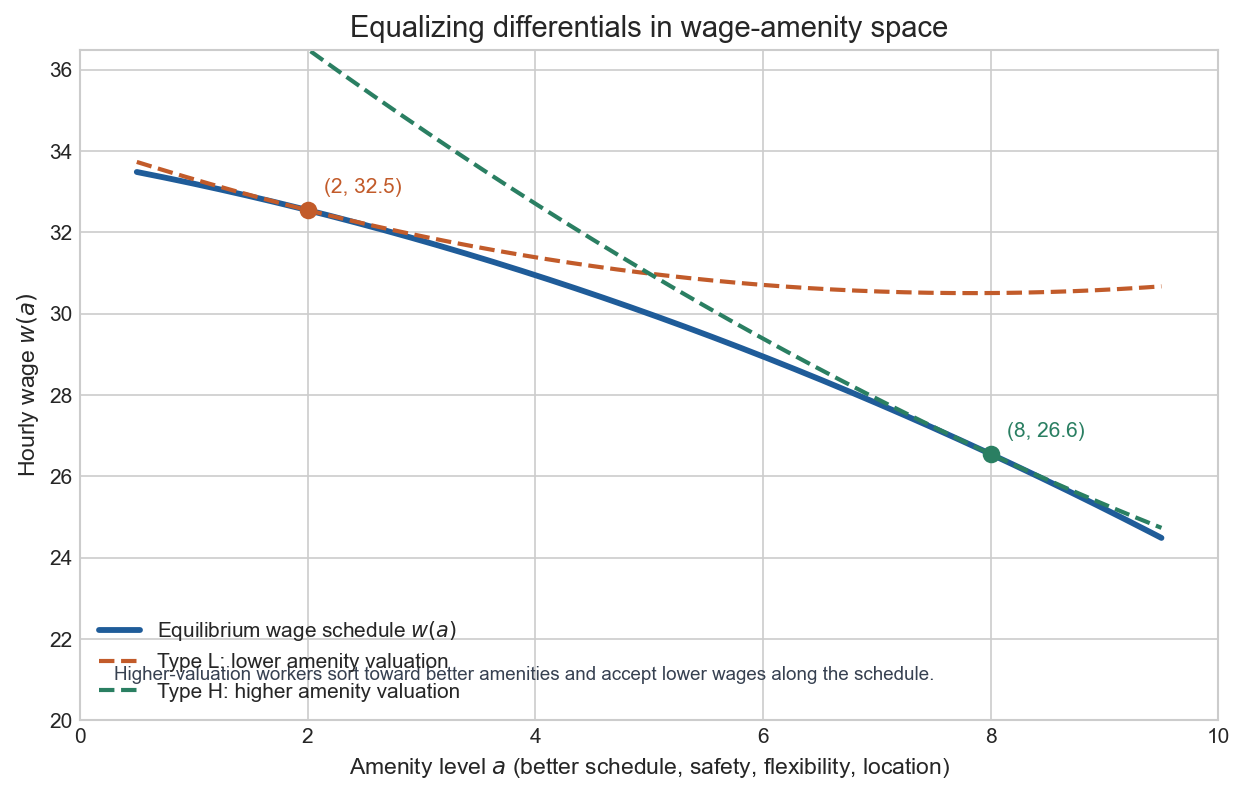
\includegraphics[height=0.74\textheight,keepaspectratio]{07-hedonic-wage-amenity-equilibrium.png}
\end{center}
\end{frame}

\begin{frame}{Firm-side amenity provision}
\[
\pi_j(a) = p_j f_j(n_j, a) - w(a)n_j - C_j(a)n_j
\]

\begin{itemize}
    \item Amenities are not free: safety, staffing slack, remote infrastructure, and schedule control all have costs or productivity effects.
    \item Firms differ in \(C_j(a)\), so the supply side of job quality is heterogeneous.
    \item The hedonic schedule reflects worker demand for amenities and firm costs of supplying them.
\end{itemize}
\end{frame}

\begin{frame}{Why hedonic wage regressions can fail}
\begin{itemize}
    \item Amenities are multidimensional and often measured badly.
    \item Workers sort on unobserved taste, skill, family constraints, and outside options.
    \item Firms bundle wages with multiple amenities and different productivity environments.
    \item Search frictions, mobility costs, and imperfect information break the clean frictionless benchmark.
\end{itemize}
\end{frame}

\begin{frame}{Modern willingness-to-pay object}
\[
U_{ij} = \beta_w w_{ij} + A_{ij}'\beta_a + X_{ij}'\gamma + \varepsilon_{ij}
\]

\begin{itemize}
    \item Discrete-choice and conjoint designs estimate marginal valuations of named job attributes.
    \item Willingness to pay for amenity \(k\) is \(-\beta_{a,k}/\beta_w\).
    \item Mas and Pallais is the Week 7 anchor because it measures explicit tradeoffs rather than inferring them from wage cross sections.
\end{itemize}
\end{frame}

\begin{frame}{Stylized willingness to pay for selected amenities}
\begin{center}
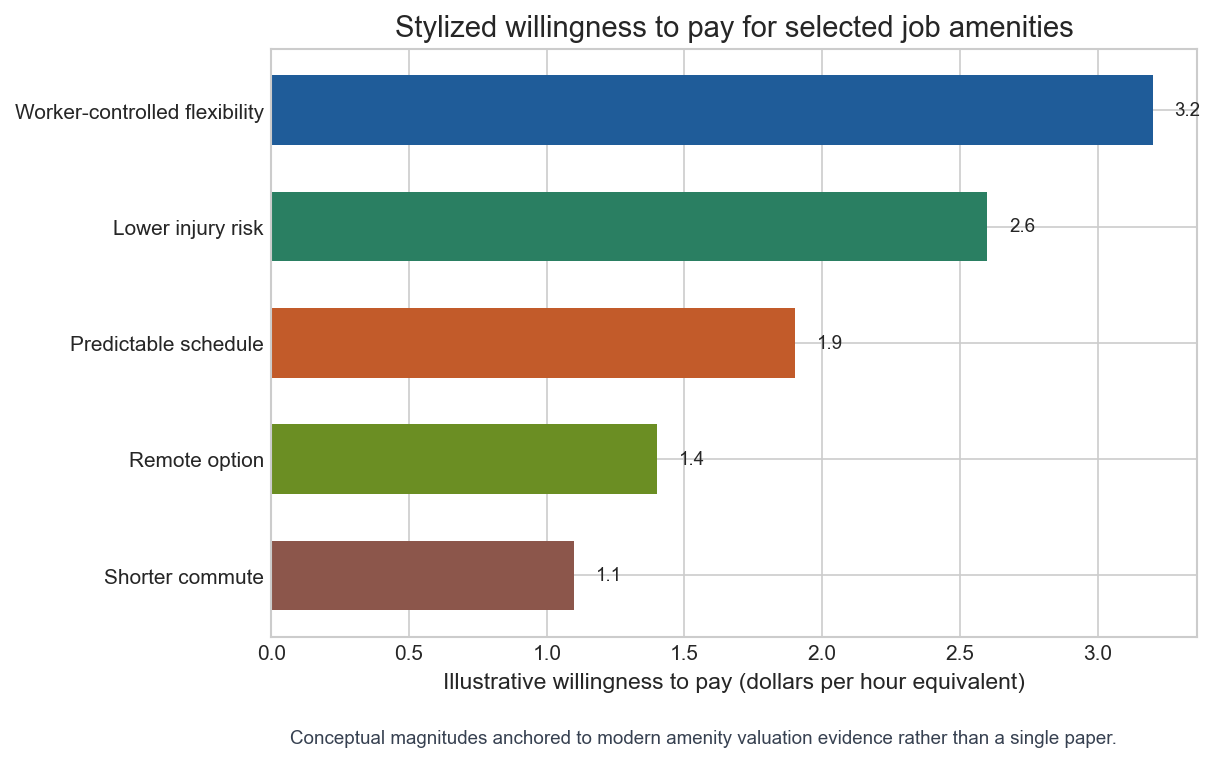
\includegraphics[height=0.74\textheight,keepaspectratio]{07-wtp-selected-amenities.png}
\end{center}
\end{frame}

\begin{frame}{Amenity taxonomy}
\scriptsize
\begin{tabular}{p{0.18\linewidth} p{0.20\linewidth} p{0.24\linewidth} p{0.22\linewidth}}
\toprule
Amenity class & Typical examples & Why it matters & Main challenge \\
\midrule
Risks and physical conditions & Injury risk, exposure, heat, noise & Canonical compensating-differentials object & Risk mismeasurement and selection \\
Schedule and timing & Predictability, advance notice, nights, overtime control & Family compatibility and stress & Bundled with occupation and firm type \\
Location and commute & Remote work, hybrid, travel, commute time & Effective value of wages and time & Commute and remote options often missing \\
Autonomy and monitoring & Break control, algorithmic monitoring, discretion & Utility and productivity both move & Hard to separate from firm quality \\
Work intensity and pace & Pace pressure, staffing ratios, emotional load & Turnover, burnout, effort & Often poorly measured \\
Prestige and social environment & Mission, culture, respect, coworker quality & Sorting and welfare & Highly subjective across workers \\
\bottomrule
\end{tabular}
\end{frame}

\begin{frame}{Empirical design map}
\scriptsize
\begin{tabular}{p{0.20\linewidth} p{0.24\linewidth} p{0.20\linewidth} p{0.24\linewidth}}
\toprule
Design & Main identifying object & Strength & Principal threat \\
\midrule
Hedonic wage regression & Cross-sectional wage-amenity slope & Broad and simple & Omitted tastes, firm heterogeneity, measurement error \\
Risk-premium studies & Compensation for injury or fatality risk & Classic policy relevance & Risk measurement and selection \\
Discrete-choice / conjoint & Willingness to pay for explicit attributes & Direct valuation of named amenities & External validity and design dependence \\
Worker-flow / revealed preference & Latent firm or job value from mobility & Uses actual choices & Rich data and stronger structure needed \\
Working-conditions bundles & Value of broader job-quality bundles & Connects to inequality & Comparability across conditions \\
\bottomrule
\end{tabular}
\end{frame}

\begin{frame}{Modern amenities, sorting, and inequality}
\begin{itemize}
    \item Maestas et al. broaden the object from a few amenities to richer working-conditions bundles.
    \item Wage inequality can overstate or understate total-compensation inequality depending on sorting patterns.
    \item High-wage firms may also offer better schedules, autonomy, and safety, which amplifies inequality in job value.
\end{itemize}
\end{frame}

\begin{frame}{Wage inequality versus total job value}
\begin{center}
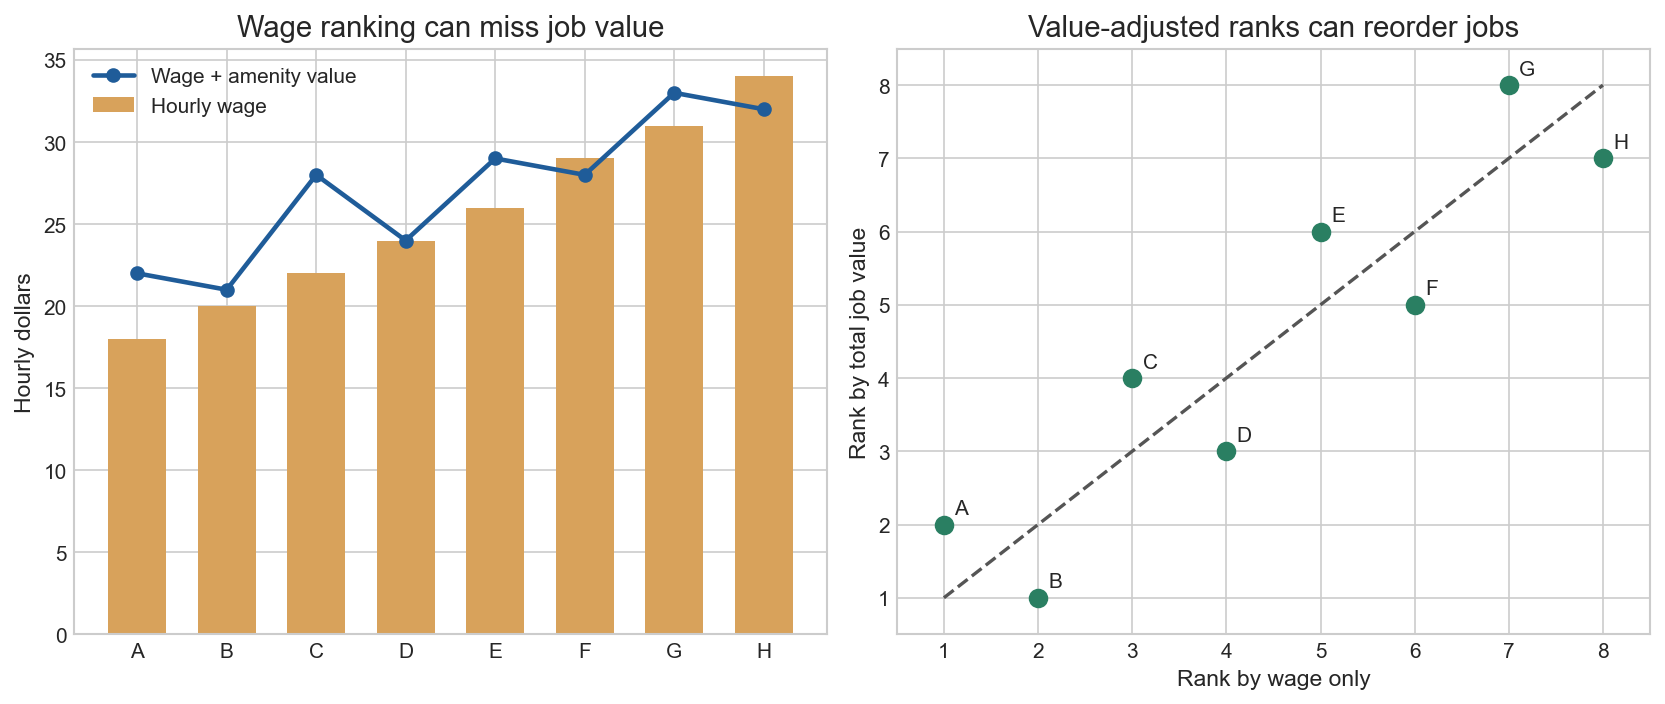
\includegraphics[height=0.74\textheight,keepaspectratio]{07-wage-inequality-total-job-value.png}
\end{center}
\end{frame}

\begin{frame}{Bridge to Week 8 and Week 9}
\begin{itemize}
    \item Week 8: wage dispersion is not the same as inequality in total job value once amenities are priced.
    \item Week 9: discrimination and segmentation may operate through access to safe, predictable, flexible, or remote jobs as well as through wages.
    \item Equalizing differences are therefore central to distributional interpretation, not a side topic.
\end{itemize}
\end{frame}

\begin{frame}{Takeaways}
\begin{itemize}
    \item Rosen's equalizing-differences framework is the benchmark for wage-amenity tradeoffs.
    \item Naive hedonic regressions are fragile because the theory predicts sorting, heterogeneity, and bundling.
    \item Modern discrete-choice and worker-flow evidence recover job value more directly.
    \item Week 7 is the hinge from wage determination to inequality and segmentation.
\end{itemize}
\end{frame}

\appendix

\begin{frame}{Appendix: optional extension block}
\begin{itemize}
    \item Risky jobs and the value of statistical life in the spirit of Viscusi and Aldy.
    \item Search-friction interpretations of compensating differentials in the spirit of Hwang, Mortensen, and Reed.
    \item Revealed-preference firm ranking in the spirit of Sorkin.
\end{itemize}
\end{frame}

\end{document}
